\documentclass[a4paper, 11pt]{article}

%%% Zeichenkodierung, Rechtschreibung und Umlaute
\usepackage[utf8]{inputenc}
\usepackage[ngerman]{babel}
\usepackage[T1]{fontenc}

%%% Mathematische Symbole, Gleichungen
\usepackage[fleqn]{amsmath}
\usepackage{amsfonts}
\usepackage{amssymb}
\usepackage{amsthm}
\usepackage{mathtools}
\usepackage{bm}
%\usepackage{colonequals} % Zusätzliche Relationssymbole

%%% Tabellen
\usepackage{tabularx}
\usepackage{array}
\usepackage{multicol}

%%% Seitenformat und -ränder
%%% -Alternative 1-
\usepackage{geometry}
\geometry{a4paper, top=25mm, bottom=20mm, left=20mm, right=20mm}
%%% -Alternative 2-
%\usepackage[headheight=110pt]{geometry}
%\geometry{a4paper,left=30mm,right=30mm, top=35mm, bottom=30mm}

%%% Seitenstile (Kopf- und Fußzeile)
\usepackage{fancyhdr}
\pagestyle{fancy}

%%% Sonstiges
\usepackage{caption} % Untertitel von Grafiken/Tabellen manipulieren
\usepackage{enumerate} % Aufzählungszeichen ändern
\usepackage{graphicx} % Standarderweiterung für Bilddateien
\usepackage{hyperref} % Hyperlinks
\usepackage{lastpage} % Berechnung der Seitenzahl
%\usepackage{polynom} % Polynomdivision
\usepackage{setspace} % Zeilenabstand
%\usepackage{textgreek} % griechische Symbole
\usepackage{tikz} % Umfassendes Tool, um Grafiken zu erstellen
\usepackage{verbatim} % Schreibmaschinen-Stil (für Code-Ausschnitte)
\usepackage{float}

%%% Eingaben (z.B. für das Deckblatt)
\newcommand{\module}{Computergrafik 2 -- Theorieaufgabe}
\newcommand{\semester}{Sommersemester 2018}
\newcommand{\finishingdate}{29.06.2018}
\newcommand{\titletext}{Blatt 3} %TODO: Nummer anpassen

%%%-- Für das Deckblatt --
\title{
	~\\[4cm]
	\textbf{
		\module\\[0.25cm]
		\normalsize \semester \\[1.5cm]
		\Huge\titletext\\
	}
}

\author{
  \vspace{3.5cm}\\
  \begin{tabular}{l}
    \textbf{Gruppe 4:}\\\hline
    Johannes Huwald \\
    Jacques Lucke\\
    Torsten Michael Schenk\\
  \end{tabular}
}

\date{
	\vfill
	Abgabedatum: \finishingdate\\
	\vspace{5mm}
	Seitenanzahl: \pageref{LastPage}
}

%%% -- Kopf- und Fußzeile --
%%% Kopfzeile linker Bereich
\lhead[\leftmark]{\textbf{\module}}
%%% Kopfzeile mittlerer Bereich
\chead[\rightmark]{\rightmark{\titletext}}
%%% Kopfzeile linker Bereich
\rhead{\textbf{zum \finishingdate}}
%%% Fußzeile
\cfoot{\thepage  \ / \pageref{LastPage}}

%%% Serifenfreie Fonts benutzen
%\renewcommand{\familydefault}{\sfdefault}

%%% Font
\usepackage{charter}

%%% Tiefe der Einrückung nach Absätzen
\setlength{\parindent}{0pt}

%%% Evtl. Änderungen des Typs einer Aufzählungsebene (z.B. zur Anpassung an das Aufgabenblatt)
%\renewcommand{\labelenumi}{\alph{enumi})}
%\renewcommand{\labelenumii}{(\roman{enumii})}
%\renewcommand{\labelenumiii}{\arabic{enumiii}.}
%\renewcommand{\labelenumii}{\textbf{-}}

\begin{document}

%%% Deckblatt
\maketitle
\thispagestyle{empty} % Keine Seitenzahl hier
\newpage

%%% Seitenzahl zurücksetzen
\clearpage
\setcounter{page}{1}

%%% Zeilenabstand
%\singlespacing
\onehalfspacing
%\doublespacing

%%%-- Eigentlicher Inhalt --
\section*{Aufgabe 1: }
Sei $p(t) = \sum_{i=0}^nb_iB_i^n(t)$ mit $b_i \in \mathbb{R}^d$ eine Bezierkurve. Für die erste Ableitung von $p$ gilt dann:
\begin{align*}
  p'(t) &= n\sum_{i=0}^{n-1}(b_{i+1} - b_i)B_i^{n-1}(t) =n\left(\sum_{i=0}^{n-1}b_{i+1}B_i^{n-1}(t) - \sum_{i=0}^{n-1}b_iB_i^{n-1}(t)\right)\\
          &= n\left(p_1(t) - p_2(t)\right)
\end{align*}
Dabei sind $p_1$ und $p_2$ zwei weitere Bezierkurven, wobei $p_1$ durch die Punkte $b_1,\cdots,b_n$ und $p_2$ durch die Punkte $b_0, \cdots, b_{n-1}$ kontrolliert wird. Nach dem Casteljau-Algorithmus gilt $p(t) = b_0^n(t)$.\\
$p_1$ und $p_2$ lassen sich analog mit $p_1(t) = b_1^{n-1}(t)$ und $p_2(t) = b_0^{n-1}(t)$ berechnen. Damit folgt für die Ableitung von $p$ weiter:
\begin{align*}
  p'(t) &= n\left(p_1(t) - p_2(t)\right) = n\left(b_1^{n-1}(t) - b_0^{n-1}(t)\right)
\end{align*}
Dies entspricht dem letzten Segment des Casteljau-Algorithmus.
\section*{Aufgabe 2: }
Gegeben sind $n$ Punkte mit einem paarweisen Abstand von $\geq \epsilon$, die sich alle in einer Zelle mit der Seitenlänge $s$ befinden. Bei der Konstruktion eines Octrees wird diese Zelle in acht Unterzellen aufgeteilt, die jeweils eine halbierte Seitenlänge besitzen. Folglich lässt sich die Seitenlänge einer dieser Zellen auf der Tiefe $d$ des Octrees mit $s_d = \frac{s}{2^d}$ berechnen. Die maximale Tiefe des Octtrees ist dann erreicht, wenn es keine Zelle gibt, in der sich mehr als ein Punkt befindet. Dies ist garantiert, wenn die Diagnonale der Zelle gleiner als $\epsilon$ ist, also $\sqrt{2 s_d} \leq \epsilon$ gilt. Es folgt:
\begin{align*}
  && \sqrt{2 s_d} & \leq \epsilon\\
  &\Rightarrow & 2\frac{s}{2^d} & \leq \epsilon^2\\
  &\Leftrightarrow & 2\frac{s}{\epsilon^2} & \leq 2^d\\
  &\Leftrightarrow & d & \geq log_2(2\frac{s}{\epsilon^2}) = log_2(2) + log_2(\frac{s}{\epsilon^2}) = 1 + log_2(\frac{s}{\epsilon^2})\\
\end{align*}
Damit beträgt die maximale Tiefe $d$ eines Octrees in diesem Szenario $d = \lceil 1 + log_2(\frac{s}{\epsilon^2}) \rceil$.
\section*{Aufgabe 3: }
Die Partitionierung des Raumes kann auch durch ein Prisma mit einem gleichschenkligen Dreieck als Grundfläche geschehen. Dann kann die Aufteilung des Raumes von dem Prisma stattfinden, indem die Höhe und Grundseite des Dreiecks halbiert werden und das daraus resultierende Prisma wie in der folgenden Abbildung viermal positioniert wird.
\begin{figure}[H]
  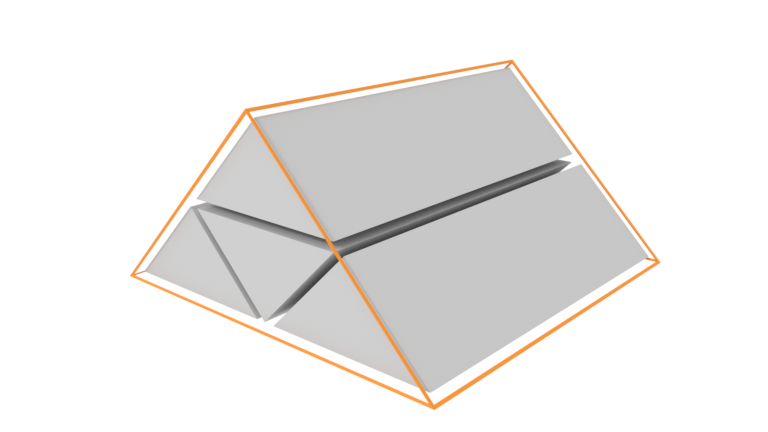
\includegraphics[width=0.7\textwidth]{prism}
\end{figure}
\section*{Aufgabe 4: }
Gegeben sind die fünf Kontrollpunkte $P_0 = (0, 0)$, $P_1 = (1, 3)$, $P_2 = (2, 1)$, $P_3 = (3, 2)$ und $P_4 = (4, 1)$.
Der Knotenvektor $T$ des B-Splines ersten Grades hat damit $m = n + k + 1 = 5 + 1 + 1 = 7$ Elemente. Mit $T = (0, 1, 2, 3, 4, 5, 6)$ folgt dann für die Basisfunktionen des B-Splines:
\begin{align*}
  N_0^1(t) &= \frac{t - t_0}{t_1 - t_0}\cdot N_0^0(t) + \frac{t_2 - t}{t_2 - t_1}\cdot N_1^0(t) = t \cdot N_0^0(t) + (2 - t) \cdot N_0^0(t)\\
  N_1^1(t) &= \frac{t - t_1}{t_2 - t_1}\cdot N_1^0(t) + \frac{t_3 - t}{t_3 - t_2}\cdot N_2^0(t) = (t - 1) \cdot N_1^0(t) + (3 - t) \cdot N_2^0(t)\\
  N_2^1(t) &= \frac{t - t_2}{t_3 - t_2}\cdot N_2^0(t) + \frac{t_4 - t}{t_4 - t_3}\cdot N_3^0(t) = (t - 2) \cdot N_2^0(t) + (4 - t) \cdot N_3^0(t)\\
  N_3^1(t) &= \frac{t - t_3}{t_4 - t_3}\cdot N_3^0(t) + \frac{t_5 - t}{t_5 - t_4}\cdot N_4^0(t) = (t - 3) \cdot N_3^0(t) + (5 - t) \cdot N_4^0(t)\\
  N_4^1(t) &= \frac{t - t_4}{t_5 - t_4}\cdot N_3^0(t) + \frac{t_6 - t}{t_6 - t_5}\cdot N_5^0(t) = (t - 4) \cdot N_3^0(t) + (6 - t) \cdot N_5^0(t)\\
\end{align*}
Diese Basisfunktionen resultieren in folgendem Graphen:
\begin{center}
  \begin{figure}[H]
    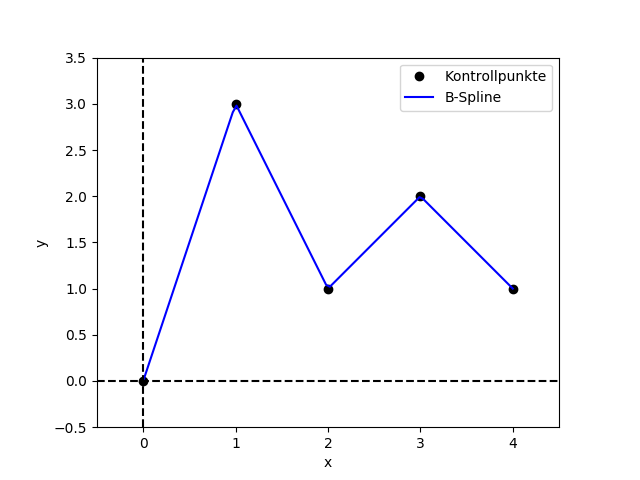
\includegraphics[width=0.7\textwidth, keepaspectratio]{splines}
  \end{figure}
\end{center}
Wie man sieht, ist die Kurve zwar stetig, allerdings nicht stetig differenzierbar. Der Grund dafür ist, dass ein B-Spline $n$-ten Grades immer genau $(n-1)$-mal stetig differenzierbar ist. Da der Grad des hier verwendeten Splines $1$ ist, ist der Graph folglich nur stetig. Im Gegensatz zu einem Polynom mit Grad $1$ (also einer linearen Funktion) ist die Steigung des Splines allerdings nicht konstant, sondern besteht aus mehreren Abschnitten mit unterschiedlicher Steigung. Dies liegt daran, dass die Basisfunktionen der Kontrollpunkte des Splines lokalen Support besitzen, die Kurve also nur in ihrer näheren Umgebung beeinflussen. So hat z.B. der zweite Kontrollpunkt $P_1 = (1, 3)$ nur im Interval $x\in [0;2]$ einen Einfluss auf die Steigung.
%\section*{Aufgabe 5:}

\end{document}
